\documentclass[11pt, a4paper]{article}
\usepackage[utf8]{inputenc}
\usepackage[left=2cm, right=2cm, top=2.5cm, bottom=2.0cm]{geometry}
\usepackage{amsmath, amssymb, amsthm}
\usepackage[english]{babel}
\usepackage{graphicx}
\usepackage[font={small,it}]{caption}
\graphicspath{ {figures/} }
\usepackage{url}
\usepackage{appendix}
\usepackage{float}
\usepackage{multirow}
\usepackage[bottom]{footmisc}
\usepackage{wrapfig}
\usepackage{subcaption}
\usepackage{titling}
\setlength{\droptitle}{-10em}  

\title{ \huge Artificial neural networks \\ 
  { \large Assigment 4: PCA and SOM }}
\author{
        Lood, Cédric \\
        \small Master of Bioinformatics
}

\begin{document}
\maketitle
%\tableofcontents

\section{Context}

In this exercise, I explored techniques of unsupervised learning using
neural networks. Specifically Principal Component Analysis (PCA) and
Self-Organizing Maps (SOM).

\section{Principal component analysis}

The idea behind PCA is to reduce the dimensionality of the data in the
input space with the hope that the lower dimensional space captures
most of the structure of the data. This is done by projecting the data
onto the eigenvectors of the covariance matrix. Once the lower
dimensionality space has been computed, another question one might try
to solve is to see whether a correct reconstruction of the datapoints
is possible.

Here we will work with a subset of the US postal service database that
consists of digitized versions of handwritten digits (16 by 16
pixels). In particular, we'll focus on the digit ``3''. On the top
left-hand side of the figure below, we view the mean ``3'' over the
500 examples we have. The right-hand side plot shows the magnitude of
the eigenvalues. The bottom left-hand side shows the plots of the
eigenvectors associated with the highest eigenvalues. As can be seen
on the ``EV 256'' plot, the curvy feature typical of a 3 seems to be
associated with the highest eigenvalue.

\begin{figure}[H]
    \centering
    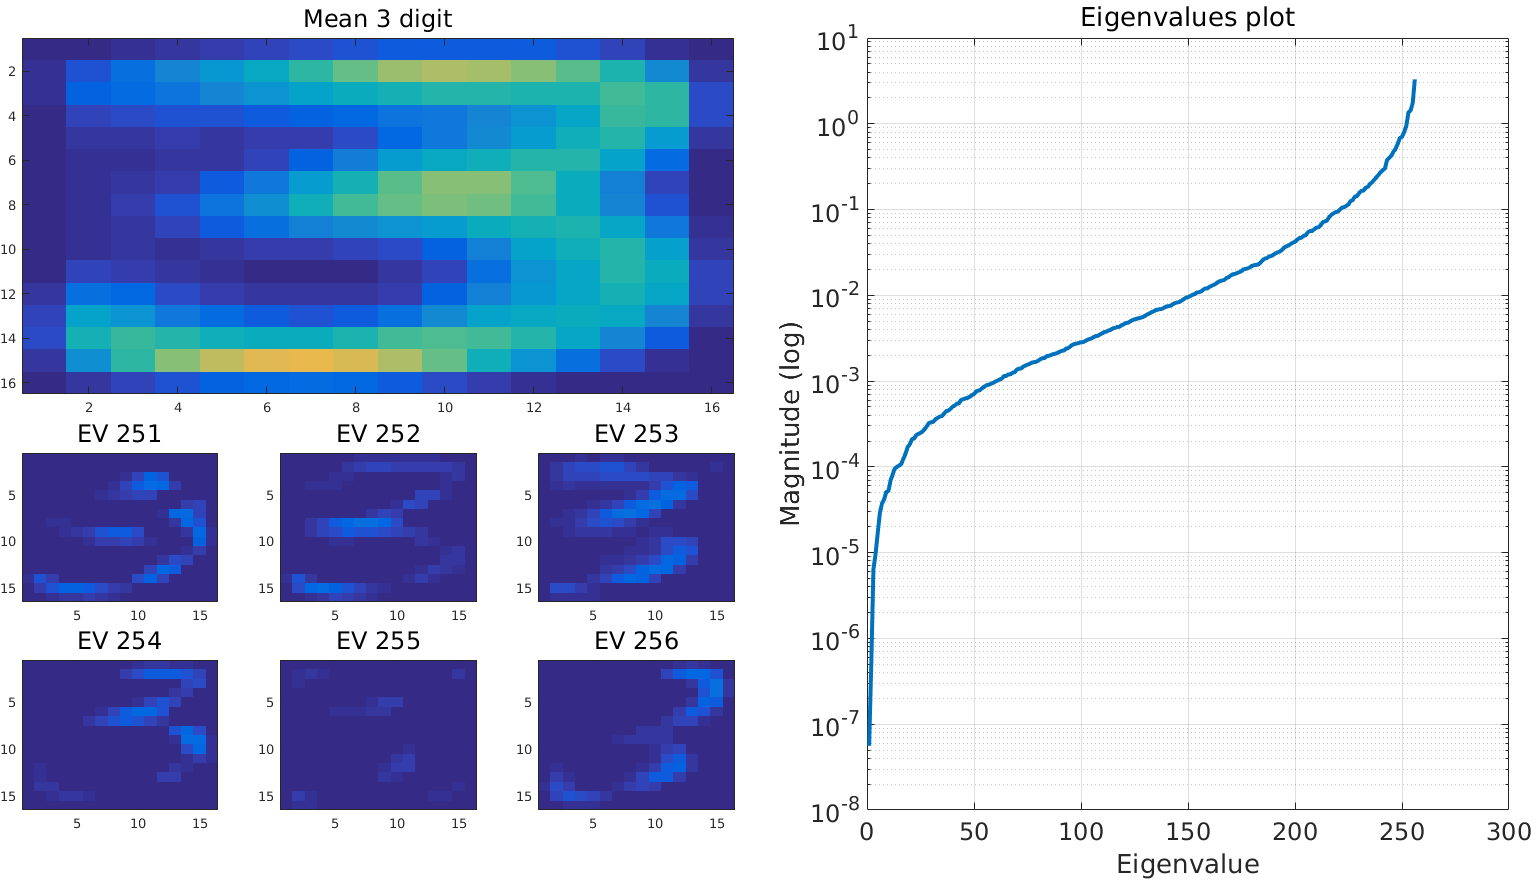
\includegraphics[scale=.25]{mean_threess.png}
    \label{fig:mean_three}
    %\caption{Left: mean 3, right: the 256 eigenvalues and their magnitude}
\end{figure}

In the next figure, you can observe the reconstruction process for 2
digits from the dataset. The rows start with the digit as it exists in
the dataset, then the next are a reconstruction of the digit based on
the first 4 principal components. As can be observed, the
reconstructed digits are much more similar than the two original
digits.

\begin{figure}[H]
    \centering
    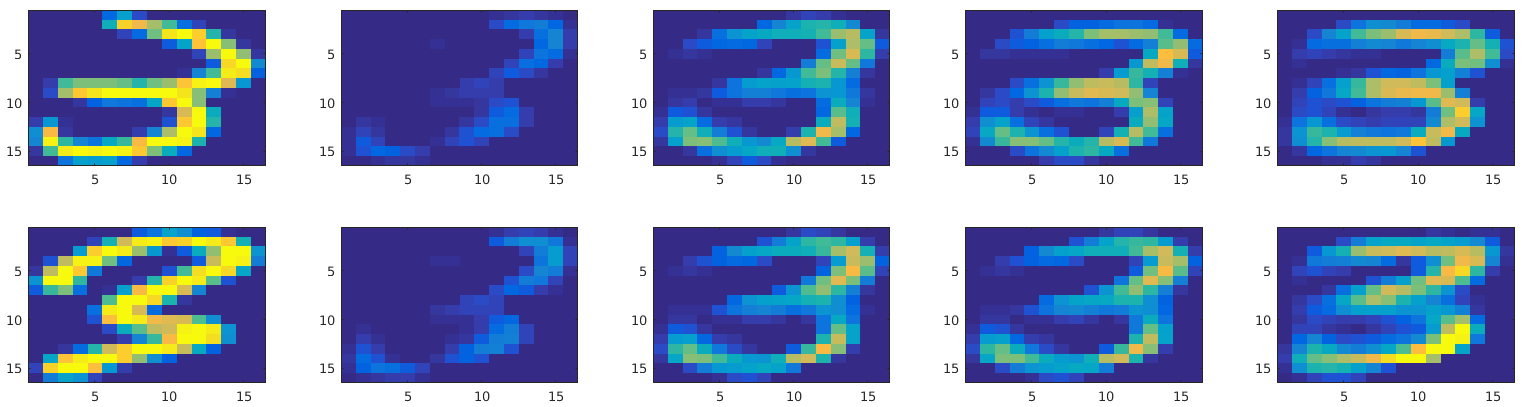
\includegraphics[scale=.20]{unsupervised_reconstructions.png}
    \label{fig:reconstructions}
\end{figure}
\begin{figure}[H]
    \centering
    \begin{subfigure}[b]{.5\textwidth}
      The graphic on the right-hand side reflects the decrease in the
      reconstruction error as the number of principal components is
      increased. One would expect that the error keeps decreasing,
      eventually reaching a value of 0, but after trying it out, I
      couldn't reach exactly 0. Visual inspection of the matrices
      containing the original dataset and the reconstructed one
      offered insights as to why that was. In the original dataset,
      many of the values are equal exactly to 0, which is not the case
      in the reconstructed dataset where the same positions are close
      to 0 but not exactly 0. I think this is due to numerical
      reasons. A comparison of the cumulative eigenvalues
      contributions and reconstruction error shows a very convincing
      correlation as can be observed on the bottom graph.
    \end{subfigure}%
    \begin{subfigure}{.4\textwidth}
      \vspace{-160pt}
      \centering
      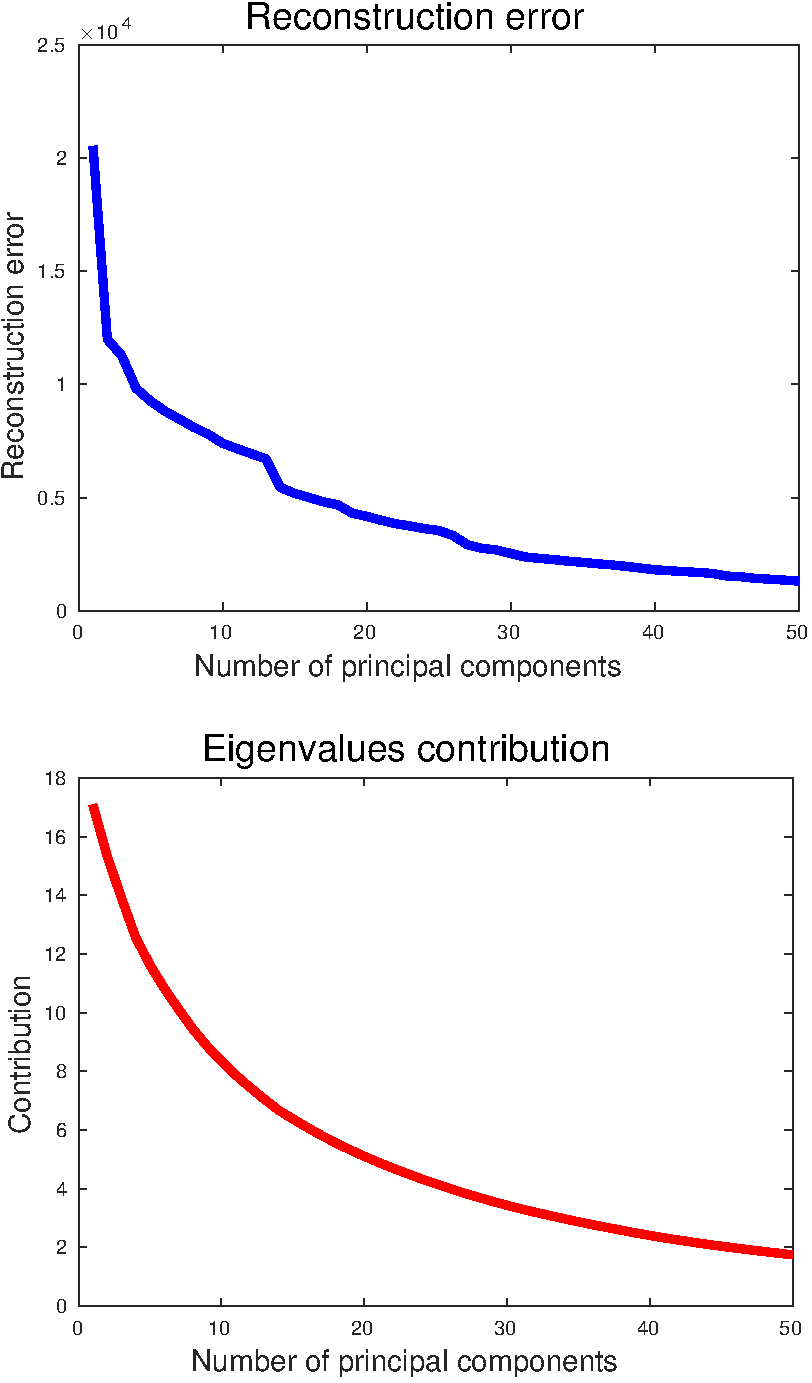
\includegraphics[width=0.8\linewidth]{unsupervised_reconstruction_error.pdf}
    \end{subfigure}
\end{figure}

\section{SOM}

% \bibliographystyle{ieeetr} 
% \bibliography{bib-db}


\end{document}
